\section{Results and discussion: The axial mass effect}
In contrast, we propose to call constant $M_{A}$ used in real form-factor $F_{A}$ ``current''. Figure~\ref{SKrates} displays the result of our calculation: ratios of the neutrino event rates caused by the QES interactions with hydrogen and oxygen nuclei in the Super-Kamiokande detector, evaluated with several values of current $M_{A}$ to ones computed with preliminary offered $M_{A}^{\mathrm{eff}}$. Figure~\ref{NOvArates} presents results for NO$\nu$A experiment in analogical way. It can be seen, that the adequate choice of the axial mass value is very important to the neutrino event rate calculations: error in count rates predicted with high-energy and hydrogen/deuterium data near NO$\nu$A energy maximum 2\,GeV achieves 6\%, using the MiniBooNE result $M_{A}=1.35$\,GeV~\cite{AguilarArevalo:2010zc} in high-entrgy region leads to approximately 30\% errors.

\begin{figure}[h!]
\begin{center}
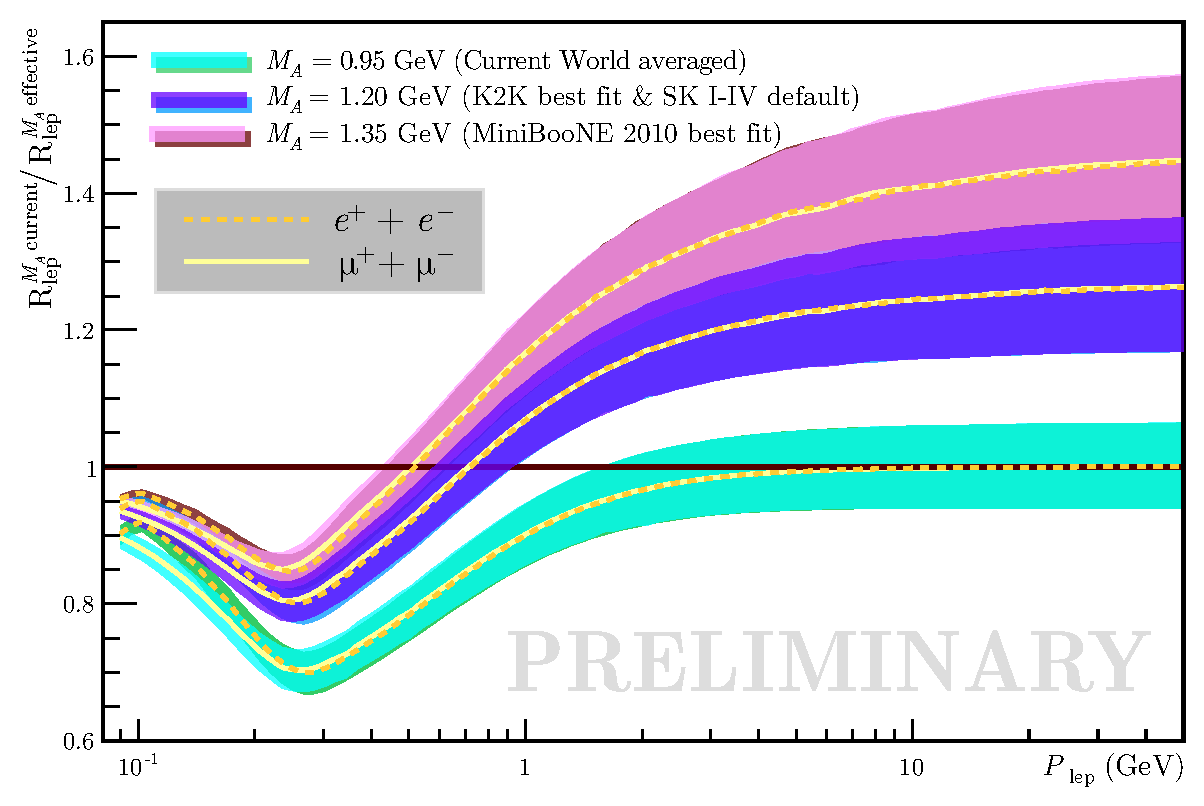
\includegraphics[width=0.6\textwidth]{./SK/cvsv2lmn_all2.eps}
\includegraphics[width=0.39\textwidth]{./SK/SK_effect_IH.eps}
\caption{\label{SKrates}Electron-like and muon-like event rates caused by the QES interactions in the Super-K detector. The rates are evaluated with several values of current $M_{A}$ and normalized to the rates calculated with $M_{A}^{\mathrm{eff}}$. The calculations are done for the normal neutrino mass hierarchy}
\end{center}
\end{figure}

\begin{figure}[htb!]
\begin{center}
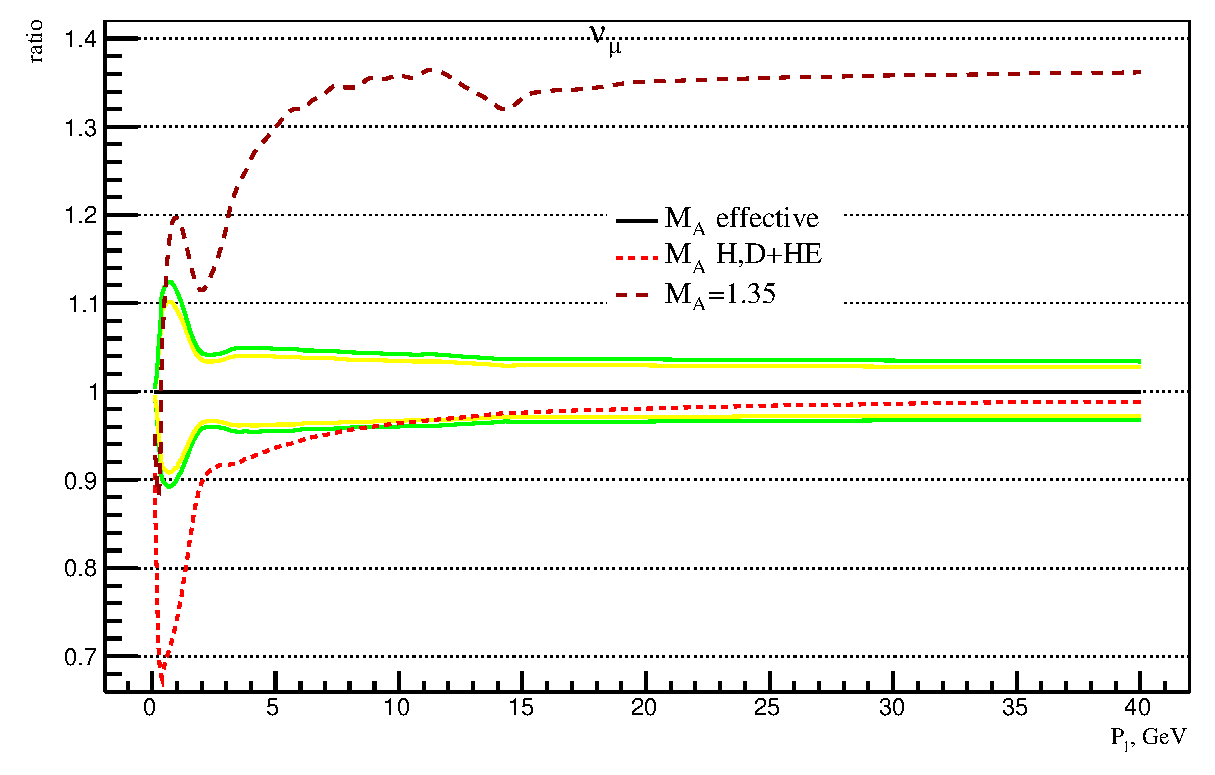
\includegraphics[width=0.45\textwidth]{./NOvA/NOvA_newflux_Scintillator_nm_n5.eps}
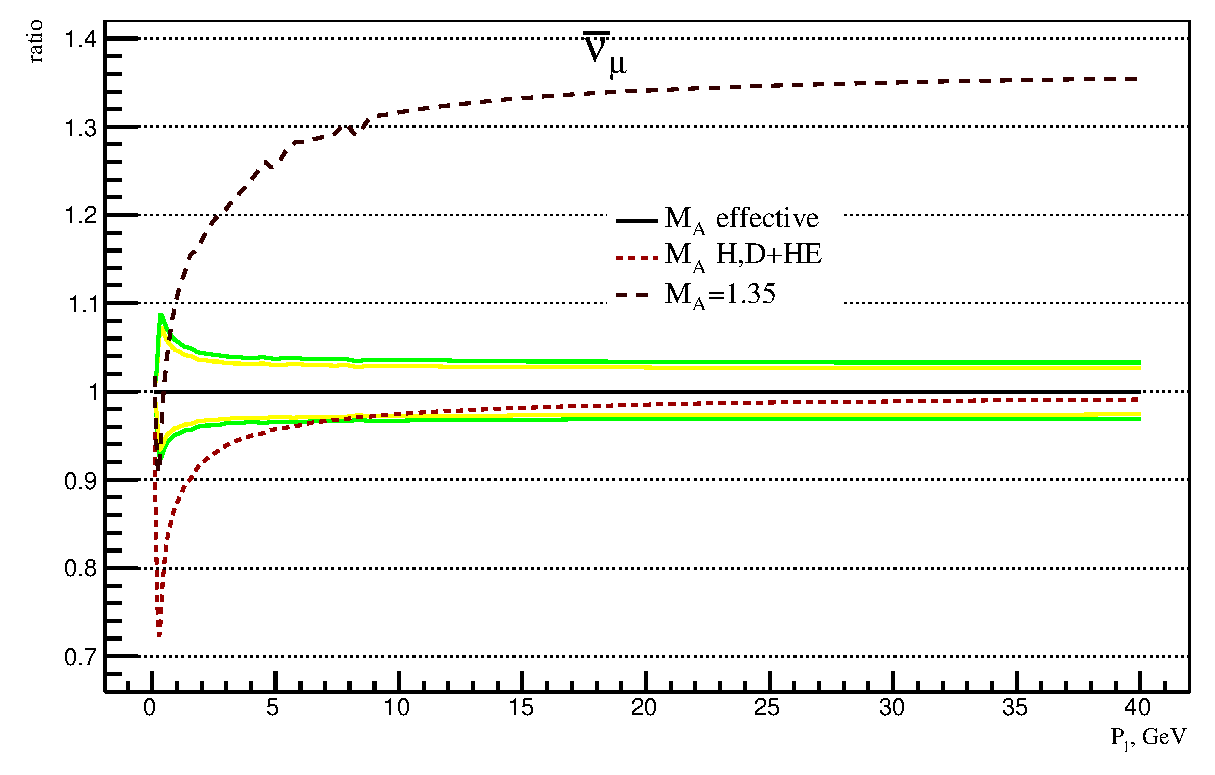
\includegraphics[width=0.45\textwidth]{./NOvA/NOvA_newflux_Scintillator_am_n5.eps}
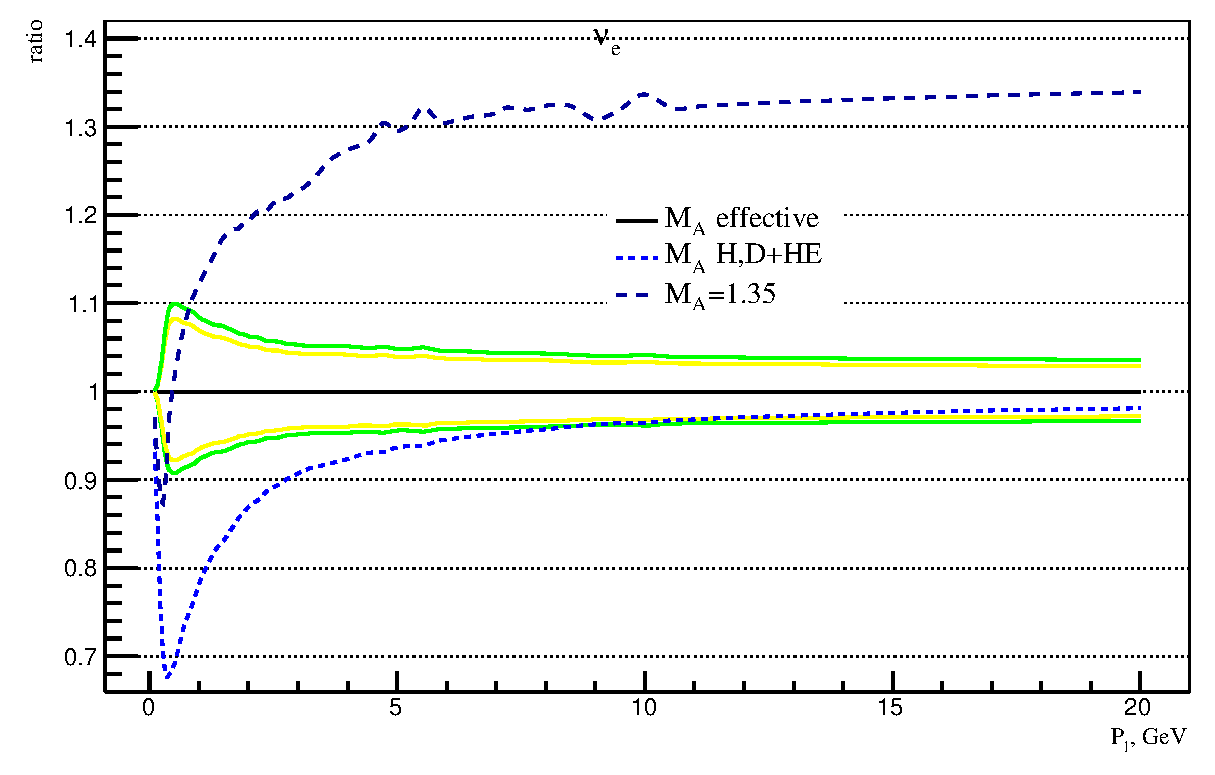
\includegraphics[width=0.45\textwidth]{./NOvA/NOvA_newflux_Scintillator_ne_n5.eps}
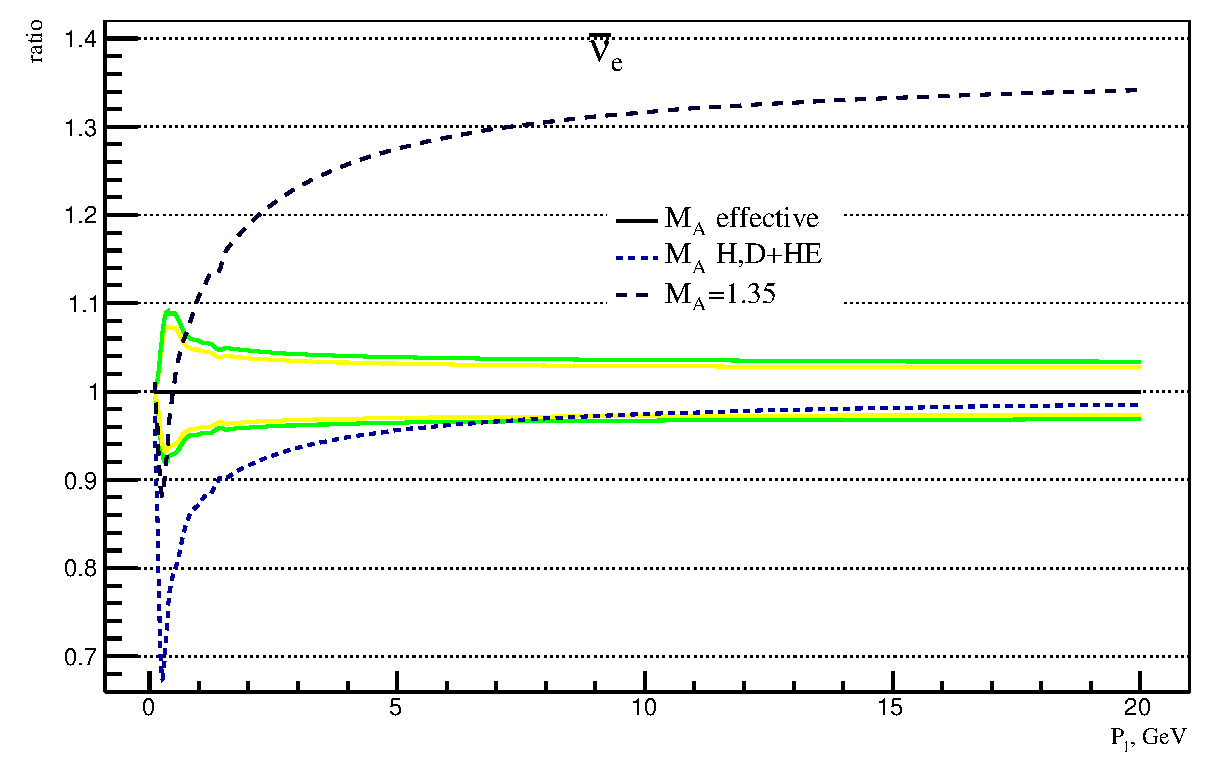
\includegraphics[width=0.45\textwidth]{./NOvA/NOvA_newflux_Scintillator_ae_n5.eps}
\caption{\label{NOvArates}Neutrino fluxes in the NOvA experiment, left-to-right: $\nu$ and $\bar\nu$-beam in Near (Far) Detector (top (bottom) panel)}
\end{center}
\end{figure}
